% ПРЕАМБУЛА

\documentclass[oneside,final,14pt]{extreport}
\usepackage[utf8]{inputenc}
\usepackage[russianb]{babel}
\usepackage{vmargin}
\setpapersize{A4}
\setmarginsrb{3cm}{2cm}{2cm}{2cm}{0pt}{0mm}{0pt}{3mm}
\usepackage{indentfirst}
\usepackage{graphicx}
\usepackage{wrapfig}
\sloppy


%НАЧАЛО ДОКУМЕНТА
\begin{document}
	
	%\setcounter{secnumdepth}{-1} % чтоб не нумеровались главы
	
	%Содержание
	\tableofcontents
	
	%Введение
	\chapter*{Введение}
	
	5.8.1 Введение должно содержать оценку современного состояния решаемой научно-технической проблемы, основание и исходные данные для разработки темы, обоснование необходимости проведения НИР, сведения о планируемом научно-техническом уровне разработки, о патентных исследованиях и выводы из них, сведения о метрологическом обеспечении НИР. Во введении должны быть показаны актуальность и новизна темы, связь данной работы с другими научно-исследовательскими работами.

От быстрого протитипирования к аддитвному производству.

Главные преимущества СЛС перед другими технологиями, это 	[vaganov corrected]
:
\begin{itemize}
    \item свойства изделий, полученных методом СЛС схожи со свойствами изделий полученных традиционными методами, такими как extrusion, injection molding, hot pressing, etc.
    \item теоретически, в технологи СЛС может быть использова любой материал, который можно получить в порошке и расплавить при increasing temperature
    \item при печати сложых продуктов не нужно дополнительных опорных элементов.
\end{itemize}

	Researches on the application of other polymers in SLS technology are very limited. In addition to polyamide, polystyrene and polycarbonate are used as a starting material for SLS.12,13
	[vaganov corrected]
	
	"Анализ современной литературы показывает, что на сегодняшний день исследования в области применения термостойких полимеров для СЛС сосредоточе-ны лишь на семействе полиэфиркетонов [Berretta S., Ghita O., Evans K. E. // European Polymer Journal, 2014. Vol. 59. P. 218–229]. На данный момент практически отсутствуют сведения об использовании других клас-сов термостойких полимеров, таких, например, как полиимиды (ПИ). Кроме того, существует ряд проти-воречивых сведений о влиянии тех или иных параметров на процесс СЛС и конечные свойства материала в целом. В связи с этим, с научной и технической точки зрения весьма перспективным представляется иссле-дование закономерностей формирования структуры при СЛС порошков ПИ, изучение процесса их сплав-ления в зависимости от свойств порошка, содержания нанонаполнителей, а также параметров СЛС.
	В ИВС РАН синтезированы термопластичные частично кристаллические ПИ гомологического ряда Р-ОДФО на основе отечественного резорцинового диангидрида Р (1,3-бис-(3,3,4,4-дикарбоксифенокси)-бензол) и четырехядерного диамина ОДФО (4,4-бис(4-аминофенокси)бифенил) методом химической (с использованием катализаторов) и термической имидизации [Юдин В. Е., Светличный В. М. // Высоко-молекулярные соединения, серия С, 2016. Т. 58. №1. С. 19]. Исследованы форма, размер частиц (фракци-онный состав ПИ порошка). Показано, что методом химической имидизации формируются порошки с более узким распределением частиц по размерам (6–10 мкм), по сравнению с термически имидизованным порошком, а при увеличении молекулярной массы и дополнительной термообработки возрастает их насыпная плотность (до 0,5 г/мл), что способствует улучшению механических характеристик изделий, формируемых по методу СЛС. Важно отметить, что с увеличением молекулярной массы ПИ наблюдается резкое возрастание вязкости его расплава, что препят-ствует слиянию частиц в процессе СЛС.
На основе ПИ порошка Р-ОДФО впервые мето-дом СЛС получены образцы в виде пленок. Исследо-ваны свойства образцов в зависимости от способа синтеза, молекулярной массы и мощности лазера и показано, что более однородная и плотная структу-ра плёнок с относительно высокими механическими характеристиками получается из порошков, синтези-руемых по методу химической имидизации.
	"[ПОЛИМЕРНЫЕ МАТЕРИАЛЫ И ТЕХНОЛОГИИ Т.4 (2018), №3, 5
Редакционная колонка — личное мнение
Полиимидные порошки для 3D-печати по методу СЛС]
	
	
	***
	Таким образом, многообещающим направлением в СЛС является использование high-performance термостабильных термопластичых полимеров и модификация полимеров with small additives наночастиц.
[SYNTHESIS AND INVESTIGATION OF NANOMODIFED POLYIMIDE POWDER FOR
SELECTIVE LASER SINTERING
Vaganov G.V.1, Didenko A.L.1, Polyakov I.V.2, Ivan’kova E.M.1, Popova E.N.1, Yudin V.E.1,2 MODERN PROBLEMS
OF POLYMER SCIENCE
Program and Abstract Book
of 14th International Saint Petersburg Conference
of Young Scientists]	


нерешенные проблемы

актуальность

+цели и задачи

	\addcontentsline{toc}{chapter}{Введение}
	
%	\chapter*{Список обозначений и сокращений}
%	СИ -- синхротронное излучение\\
%	Р-ОДФО -- наш полимер\\
%	WAXS -- широкоугловое рассеяние\\
%	и тд и тп
	
	%Теоретическая глава
	\chapter{Теория}
	\section{Селективное лазерное спекание}
\subsection{Технология}
Процесс печати изделия изображен схематически на рис. \ref{fig:printer}.\\
Описание. 

\begin{figure}[h]
    \centering
    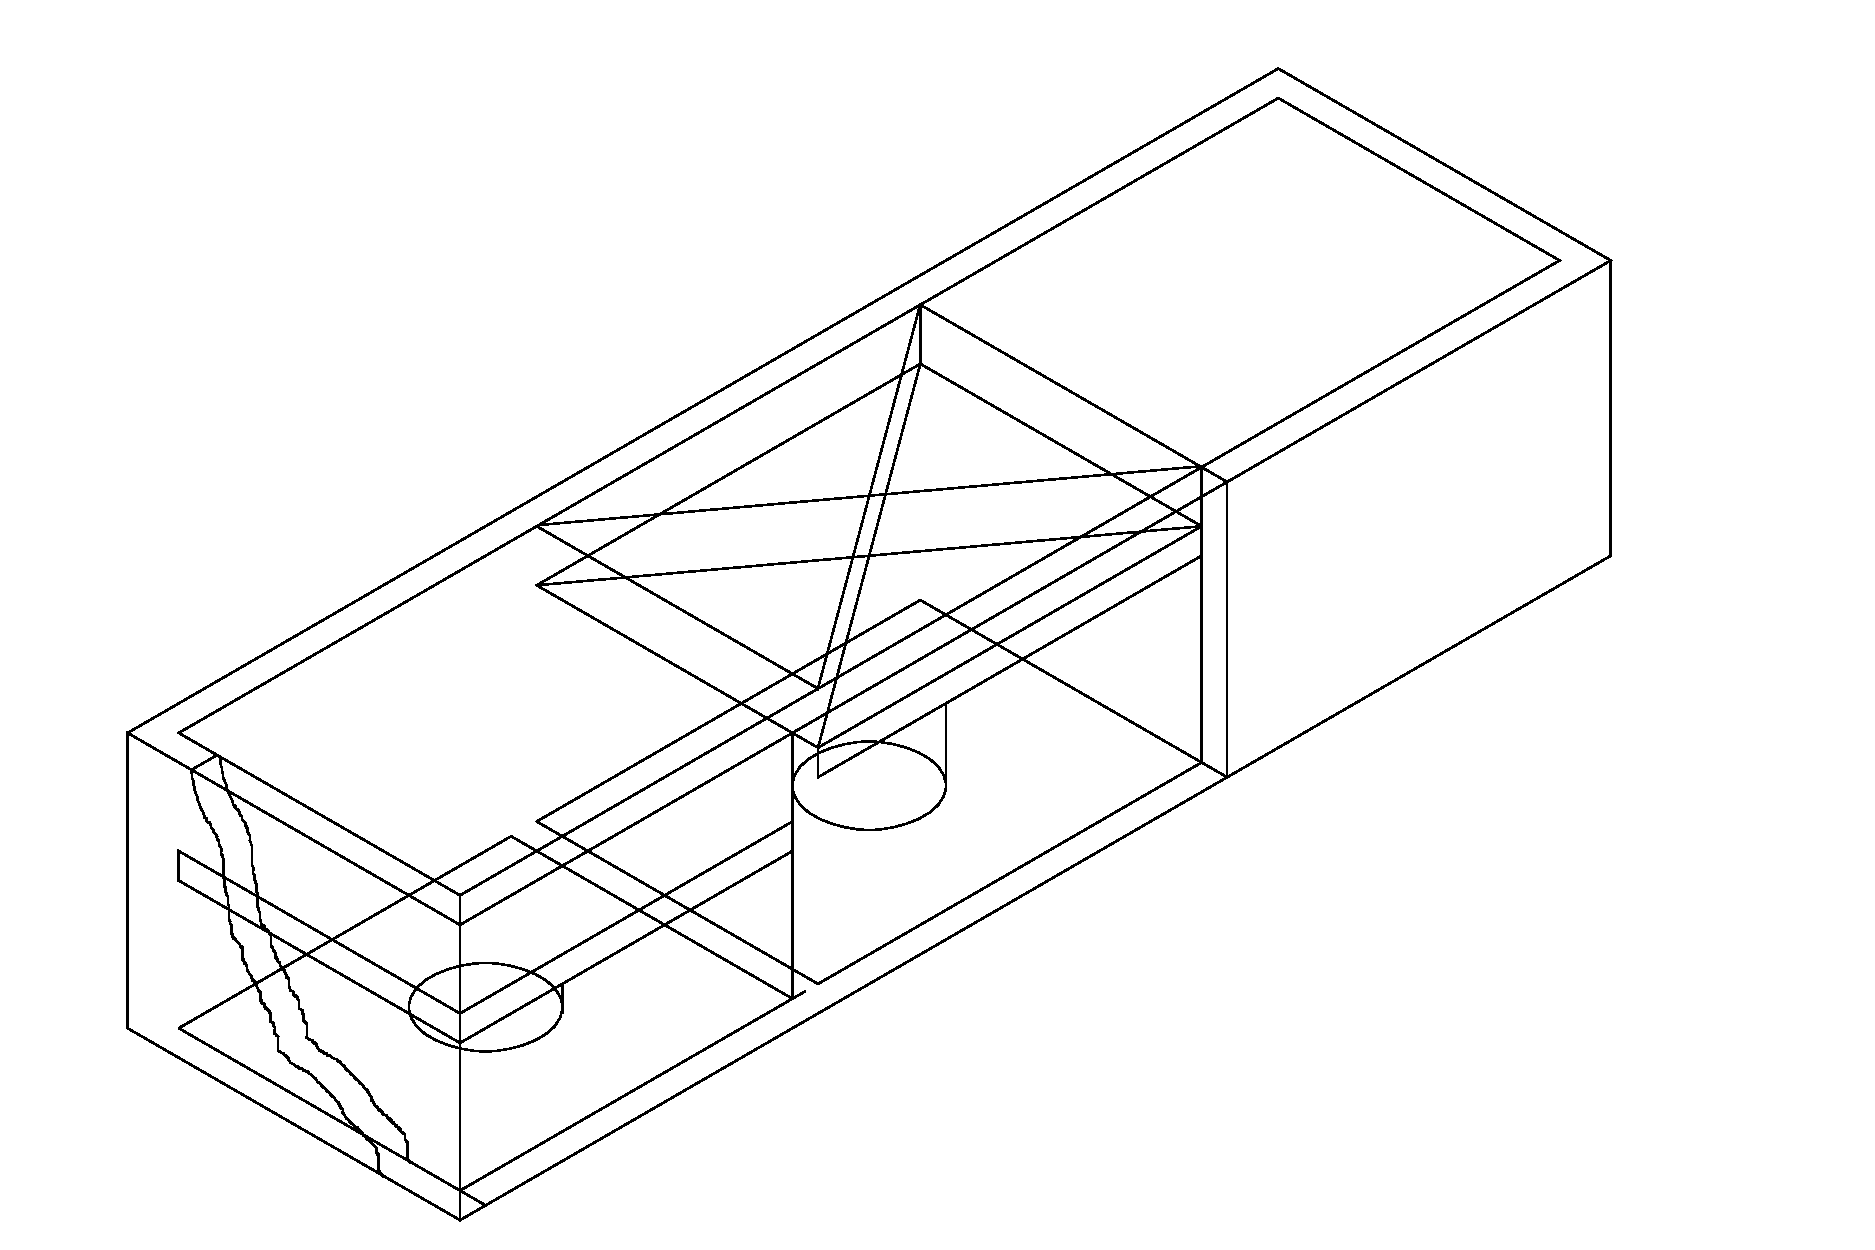
\includegraphics[width=\linewidth]{fig/sls-30deg.pdf}
    \caption{Caption}
    \label{fig:printer}
\end{figure}
анизотропия, слои\\
чтоб успевало спекаться (не спалвляться!!!)\\
Спекание отличается о сравнения

\subsection{Модель}
Высокая интенсивнсть лазерного излучения позволяет быстро нагревать небольшие участки материала, создавая большие градиенты температур \cite{sls-sim2016}.
\\

The simulation
results showed a big difference in the temperature distributions
of composite powders, especially in terms of melting depth.\\
The experimental investigation became more
efficient due to the process predictions. The accuracy of the model
was validated by the microstructures of PA, PA/CF and PA/NaCl.
With the increasing research into various composites, this numerical
method can be further used to adopt appropriate processing
parameters for the production of functional parts and then engender
significant time and material savings.
\section{Характеристиики полимеров для СЛС}
Кочены характеристики изделия, полученного по технологии СЛС, во многом зависят от от свойств начального порошка (морфология, размер, распределние размеров, объемная плотность, термические свойства, вязкость, поверхностное натяжение )  и параметров спекания (мощность лазера, скорость сканирования, диаметр пятна излучения лазера ). Морфология частиц определяет пространственное расположение частиц порошка (stacking degree) относительно друг друга. Сферические (с гладкой поверхностью) частицы имеют высокую плотность упаковки. Они обеспечивают  сыпучесть in systems of applying the material with minimal resistance. В добавок, сферические частицы хорошо связываются в процессе спекания.Показано, что 
during the transition from powder particles with predominantly spherical morphology to particles of irregular shape of the same material, the elastic modulus decreases by almost 40 \%. 
(найти ссылку ,потом перевести).
Таким образом, сферический частицы с хорошей сыпучестью и высокой плотностью упаковки представляют идеальные характеристики стартового пороша для испольщования в СЛС.\\
В то же время использование частиц неправильной формы с большой вариацией в размерах ведет к созданию продуктов с более высокими механическими характеристиками в сравнении с использованием mainle сферических частиц с узким распределением размеров.

\subsection{Тепловые и механические параметры}
первая глава из
\cite{termopols}


\subsection{"Тонкая" Структура}
Что ее характеризует
Поскольку кристаллические области в этих полимерах формируются из длинных цепей, их кристаллизация сложна и сильно чувствительа к маленьким изменениям в полимерной (compostion), добавкам, температуре и механическим воздействиям.\\
Не все полимеры кристаллизуются, а те, что кристаллизуются, редко делают это полностью: только небольшая часть crystallizable цепей incorporated into crystalline domains, а остальные segregate into amorphous domains. Степеь кристалличности и характеристики кристаллических domains являются самыми важными морфологическими характеристиками, которые определяют физические свойства такие как плотность, mechanical strength, processability, permeability and degradability частичнокристаллического полимера.\\
Степень кристалличности типичного полимера варьируется в пределах от 10 до 80 \%. Сравните с металлами, которые, за исключением металлических стекол, почти всегда полностью кристалличны, и ceramics, которые или полностью кристалличны, или аморфны.\\ \cite{cryst3} или \cite{cryst1}






\subsection{Полиэфиримиды ряда R-BAPB }
		
	\begin{figure}[h]
	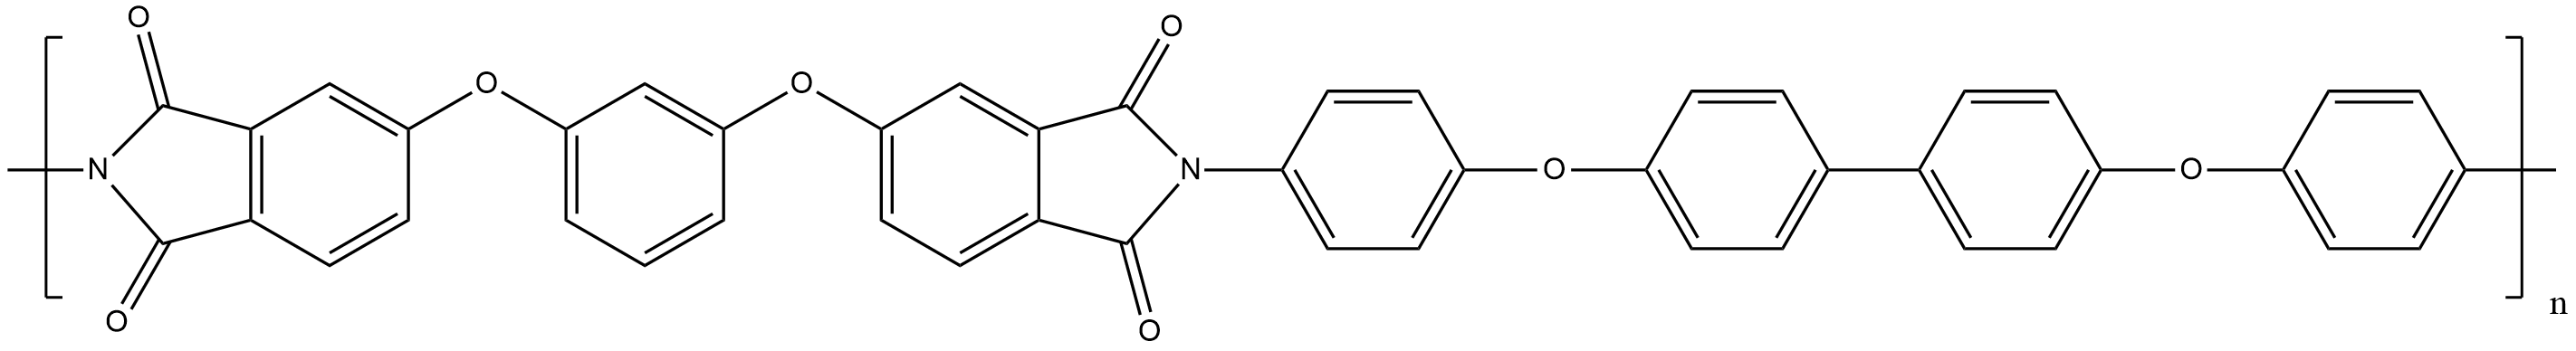
\includegraphics[width=\textwidth]{fig/formula.png}
	\end{figure}
	структура

Что следует из первичной структуры, термостойкость, особенности, пригодность для СЛС, перспективность

Данные по композитным добавкам

характеристики - все что измерили в ИВС

Что еще нужно выясеить

\subsection{Проблемы}



\section{Кристаллическая структура полимеров}
Кристаллическая структура полимеров менее идеальна чем кристаллы соединений с меньшей молекулярной массой. Как правило полимерные материалы находятся в метастабильном состоянии, то есть являются частично кристаллическими и частично аморфными. Большинсво полимеров частичнокристалличны по структуре, кристаллические структуры часто формируются при охлаждении расплава, что контролирует механические и физические свойства частичнокристаллических полимеров. Ввиду высокой вязкости полимерных расплавов, полимеры кристаллизуются очень медленно при температурах ниже температуры плавления ($T_m$), даже при высоком переохлаждении (high supercooling)
\\
Кристаллическая структура и степень кристалличости зависят от молекулярной структуры полимера, условий (growth
conditions), присутствия инородых частиц в решетке, температуры кристаллизации, скорости охлаждения и т.д.\\
Они могут быть оценены из рентгеновской дифракции, измерений плотности, термического аналища и т.д.

\subsection{Кристаллиты}
Морфологии полимерных кристаллов можно условно поделить на ламеллярные и фибриллярные кристаллы. В процессе ламеллярной кристаллизации, направление роста перпендикулярно направлению цепи, возникает складываение цепочки.Во время фибриллярной кристаллизации, наплавление роста кристалла совпадает с направление цепи, и в решетке кристалла возникают highly extended chain conformations. Такие материалы имеют высокие механические свойства. Кристаллизация существенно меняет физические и механические свойства полимерных систем. \\

Studying the crystallization
behavior, though complicated, is necessary mainly in relation to the physical and
mechanical properties of polymers. If crystallization would be absent in polymer
systems, then the whole mechanical performance of polymers depends on the glass
transition temperature (Tg). If glass transition is the only determining factor for the
properties of the polymers, then polymers such as polypropylene (PP) and PE
would have been rubbers at ambient temperature. However, in these polymers,
due to crystallization, the stiffness is retained at acceptable and controllable values
up to the melting temperature (Tm).\\
Multiphase polymer systems commonly consist of polymer blends, composites,
nanocomposites, interpenetrating polymer networks, block copolymers, and polymer
gels. Crystallization in multicomponent polymer-based systems represents the main
physical characteristic that allows for control of the material properties.\\
The presence of nanoparticles
can also limit themotion ofmolecular chains, resulting in suppression of the crystalline
perfection and crystallinity of polymer crystals.\\
Crystallization is a first-order transition and a thermal process in polymers. The
polymer chains are aligned and folded together to form an ordered chain region,
which is called lamellae. The lamellae are composed of spherical aggregates called
spherulites. The crystallization process changes the density, symmetry, and phase
transition and thus controls the properties of the end products. Crystallization
commonly proceeds by nucleation of a fiberlike structure followed by lamellar
structure formation. The spherulites grow away from a nucleation site.\\
Nowadays polymer composites are commonly used in aerospace, sport goods, automobiles,
industrial equipment, etc. Polymer composites are polymer-based matrix
with some form of materials embedded in the matrix, as reinforcements.\\
Polymer composites are classified on the basis of the size of filler particles into
microcomposites and nanocomposites.\\
(Это в планы на будущее)
Many experimental techniques can be used to study the crystallization
kinetics of nanocomposites. The most common techniques used to study the
crystallization kinetics in the nanocomposites are DSC, optical microscopy, and
WAXD.\\
The crystallization
kinetics of polymer composites and nanocomposites gained great interest due to the
fact that fillers act as an effective nucleating agent in the polymer matrix. With the
advancement of nanotechnology, the focus is now shifting toward understanding
the crystallization properties of materials in nanodimensions and thereby tune the
properties for diversified tailored application.\\

Это все из \cite{cryst1}

	\begin{wrapfigure}{r}{0.5\textwidth} 
\vspace{-20pt}


  \begin{center}
    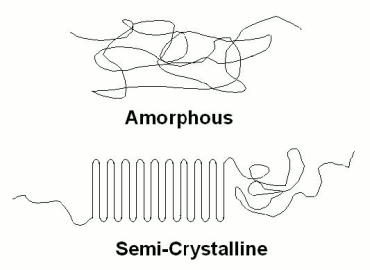
\includegraphics[width=0.4\textwidth]{fig/crystal-1.png}
    \caption{Как цепочки складываются в ламели}
    \label{fig:crystal-1}
  \end{center}
  \vspace{-20pt}
  \vspace{1pt}
\end{wrapfigure}



\begin{figure}[h]
    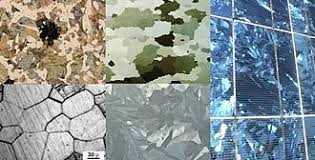
\includegraphics[width=\textwidth]{fig/crystallites.jpg}
    \caption{Типы кристаллитов}
    \label{fig:crystallites}
\end{figure}



\subsection{Частичная кристалличность}
Properties of the semicrystalline polymers can be understood, for the most part,
using a simple two-phase model that assumes that the two phases, the crystalline and
the amorphous, can be easily distinguished. If an intensive property $\phi$ (e.g., specific
volume, specific heat) of the crystalline and amorphous phases, $\phi$ c and $\phi$a, respectively, can be measured, and if we assume that contributions of the two phases
are additive, then
\[ 
\phi = \phi_c x + \phi_a(1-x)
\]
where x is the fraction of the crystalline phase, which ideally is the mass fraction
(x\_m) but depends somewhat on the technique (это из \cite{cryst3})
The
smallest organized units of polymer chains are crystallites or lamellae. These further
assemble to form fibrils and spherulites. The occurrence of spherulites and fibrils can
be used to identify if the polymer is crystalline or not, and to measure local crystallinity\\
Units such as lamellae and fibrils (nanometers) can be visualized only by
transmission electron microscopy, whereas larger units such as spherulites (micrometers)
can be monitored by optical microscopy. Crystalline features can also be
imaged using contact mode atomic force microscopy, for instance, by correlating
the surface roughness and local stiffness to crystallinity. Studies of the crystalline
growth, formation of fibrils, and growth of spherulites lead to a better understanding
of the crystallization behavior of polymers.
	
	\begin{wrapfigure}{r}{0.5\textwidth} 
\vspace{-20pt}
  \begin{center}
    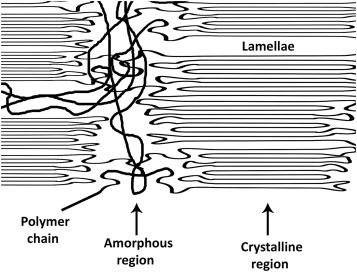
\includegraphics[width=0.4\textwidth]{fig/crystal-2.jpg}
    \caption{К определению кристалличности полимеров}
    \label{fig:crystal-2}
  \end{center}
  \vspace{-20pt}
  \vspace{1pt}
\end{wrapfigure}	

The two-phase model implied in Eq. (3.1) is only an approximation because
there can be a continuum of structures from large, defect-free single crystals to
the truly amorphous domains with liquid-like order. Because of the restrictions
imposed by long polymer chains, defects are invariably present in the crystal lattice,
and the polymer crystallites are small and disordered.\\
Conversely, the amorphous
domains possess some degree of positional and orientational correlations, and there
is experimental evidence for both rigid or ordered and soft or fluid amorphous phases\\
it may not always be possible to distinguish between the signatures
of the crystalline and amorphous phases. Nevertheless, a two-phase model with
an approximate crystalline phase and an amorphous phase, and sometimes an additional
ordered phase, mostly due to oriented amorphous domains, is often used.\\



\subsection{Влияние на макроскопические параметры}





	
	
	%Экспериментальная глава
	\chapter{Эксперимент}
	

	\section{Материалы}
	
	
	
	\section{РСА}
	
	\subsection{Почему этот метод}
	когерентность и здоровая статистика
	
	
	\subsection{Схема эксперимента}
	
	\begin{lstlisting}[language=Python, caption=Python example]
import numpy as np
 
def incmatrix(genl1,genl2):
    m = len(genl1)
    n = len(genl2)
    M = None #to become the incidence matrix
    VT = np.zeros((n*m,1), int)  #dummy variable
 
    #compute the bitwise xor matrix
    M1 = bitxormatrix(genl1)
    M2 = np.triu(bitxormatrix(genl2),1) 
 
    for i in range(m-1):
        for j in range(i+1, m):
            [r,c] = np.where(M2 == M1[i,j])
            for k in range(len(r)):
                VT[(i)*n + r[k]] = 1;
                VT[(i)*n + c[k]] = 1;
                VT[(j)*n + r[k]] = 1;
                VT[(j)*n + c[k]] = 1;
 
                if M is None:
                    M = np.copy(VT)
                else:
                    M = np.concatenate((M, VT), 1)
 
                VT = np.zeros((n*m,1), int)
 
    return M
\end{lstlisting}
	
	
	\subsection{Обработка резлультатов}
	
	\paragraph{интегрирование распознавание пиков}
	че получили:
		\begin{figure}
    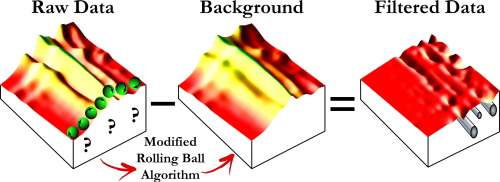
\includegraphics[width=\textwidth]{fig/rolling-ball.jpg}
    \caption{Принцип работы алгоритма}
    \label{fig:rolling-ball}
\end{figure}
	
	\paragraph{Rolling-ball}
	погрешности, чем хорошо, почему он, какие еще бывают
	
	А код - в приложении!
	
	\begin{figure}
    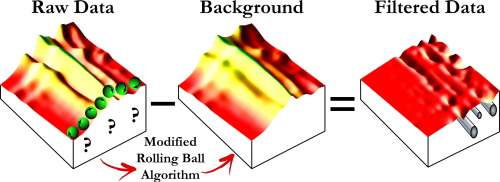
\includegraphics[width=\textwidth]{fig/rolling-ball.jpg}
    \caption{Принцип работы алгоритма}
    \label{fig:rolling-ball}
\end{figure}

    \paragraph{фиттинг}

\begin{figure}
    \centering
    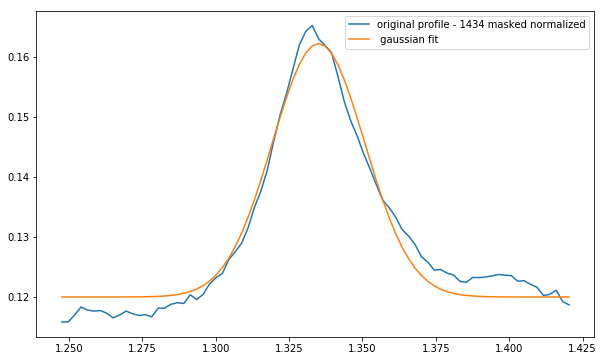
\includegraphics[width=\linewidth]{fig/gauss-fit.png}
    \caption{Аппроксимация формы пика по разным моделям}
    \label{fig:my_label}
\end{figure}
	
	\paragraph{Карты кристалличности}
	
	\begin{figure}[ht]\center
\begin{tabular}{cc}
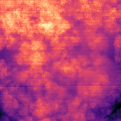
\includegraphics[width=0.5\linewidth]{fig/map-1.png}
&
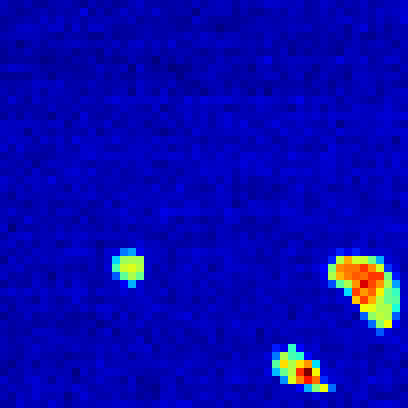
\includegraphics[width=0.5\linewidth]{fig/map-2.png}
\end{tabular}
\caption{Карты кристалличности}
\end{figure}
	
	

	
	
	
	Свойства и результаты прочих исследований:
	[Vaganov corrected]
	
	%Результаты
	\chapter{Результаты и обсуждение}
		\section{Получение и первичная обработка данных}

\subsection{Интегрирование}	
	
			\begin{wrapfigure}[17]{l}{0.6\linewidth}
\singlespacing
\vspace{-35px}
%  \begin{center}
    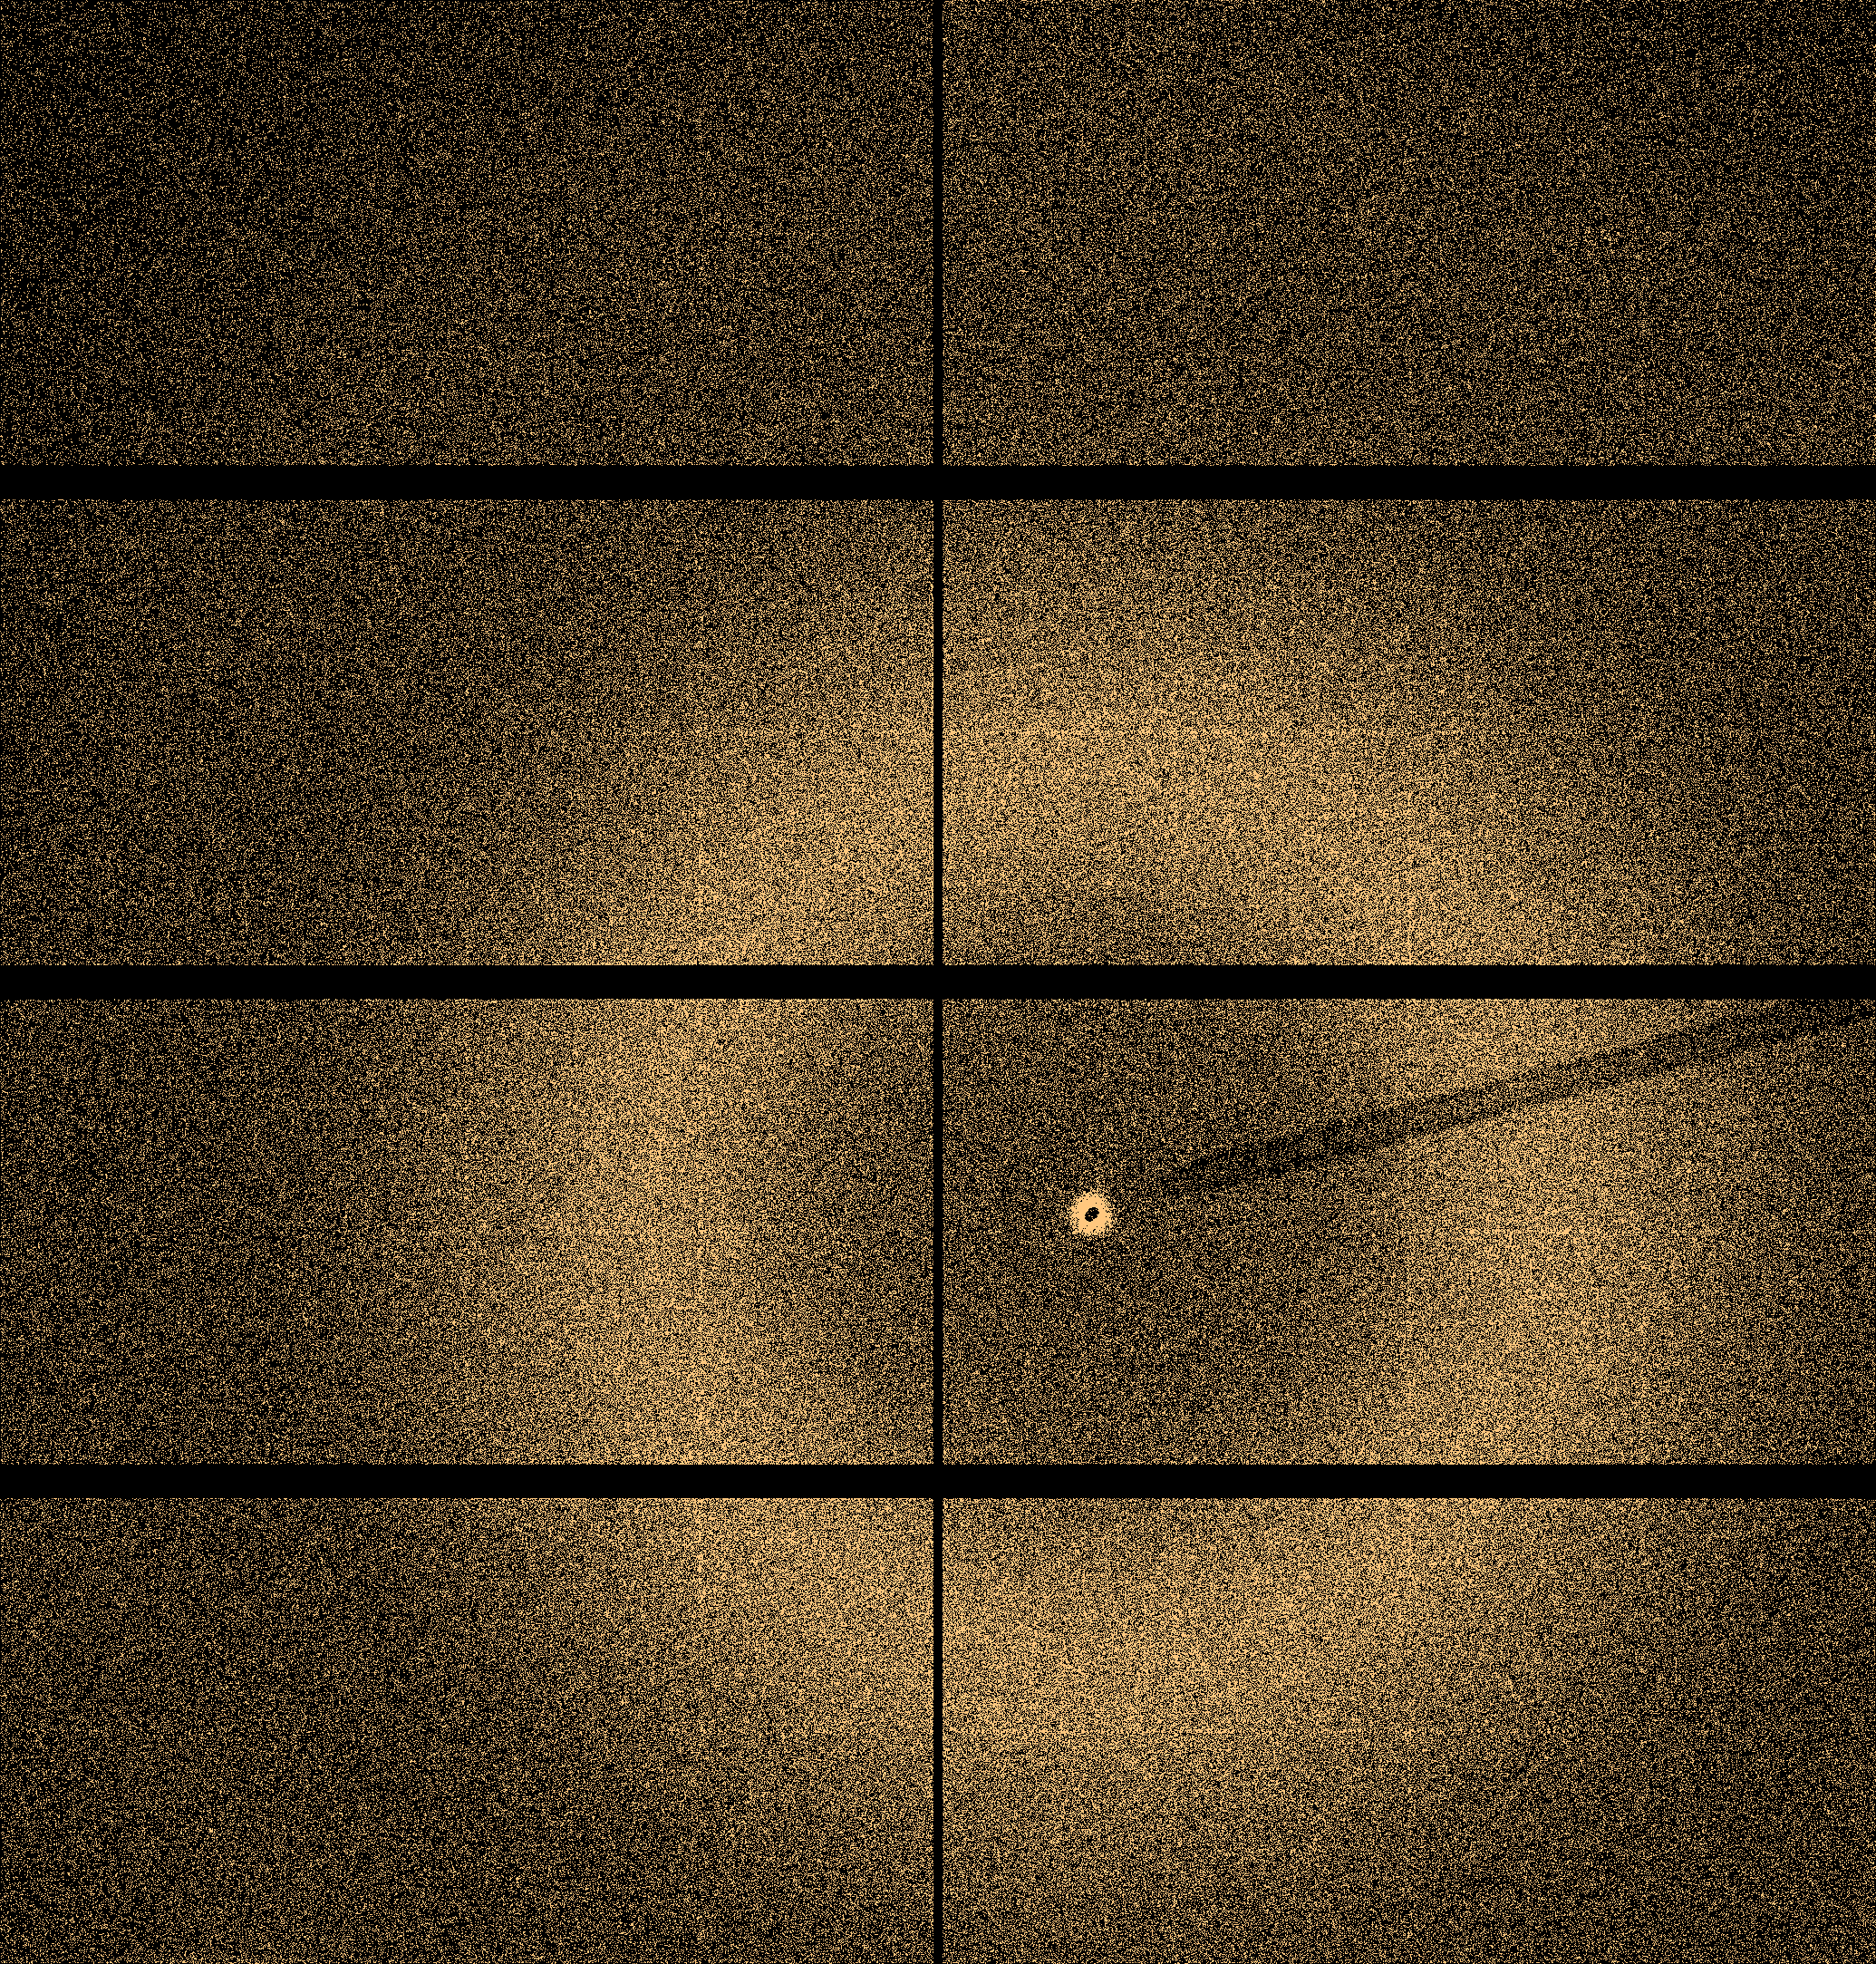
\includegraphics[width=0.9\linewidth]{fig/obj.png}
    \vspace{3px}
    \caption{Изображение с 2D~-детектора. Черные области соответствуют промежуткам между элементами детектора, затемненная облась справа  - тень от заслонки}
    \label{fig:difractogram}
%  \end{center}
\end{wrapfigure}
	
	
	Детектирование картин дифракции при сканировании образца наноразмерным пучком рентгеновского синхротронного излучения производится с шагом 1 мкм. 
	Это позволяет установить, что изучаемые порошки и пленки не являются однородными, а имеют как чисто аморфные, так и частично-кристаллические участки.
	Типичное изображение, получаемое на детекторе для единичного измерения, представлено на рис. \ref{fig:difractogram}. 
	
	\begin{figure}[t]\center
\begin{tabular}{cc}
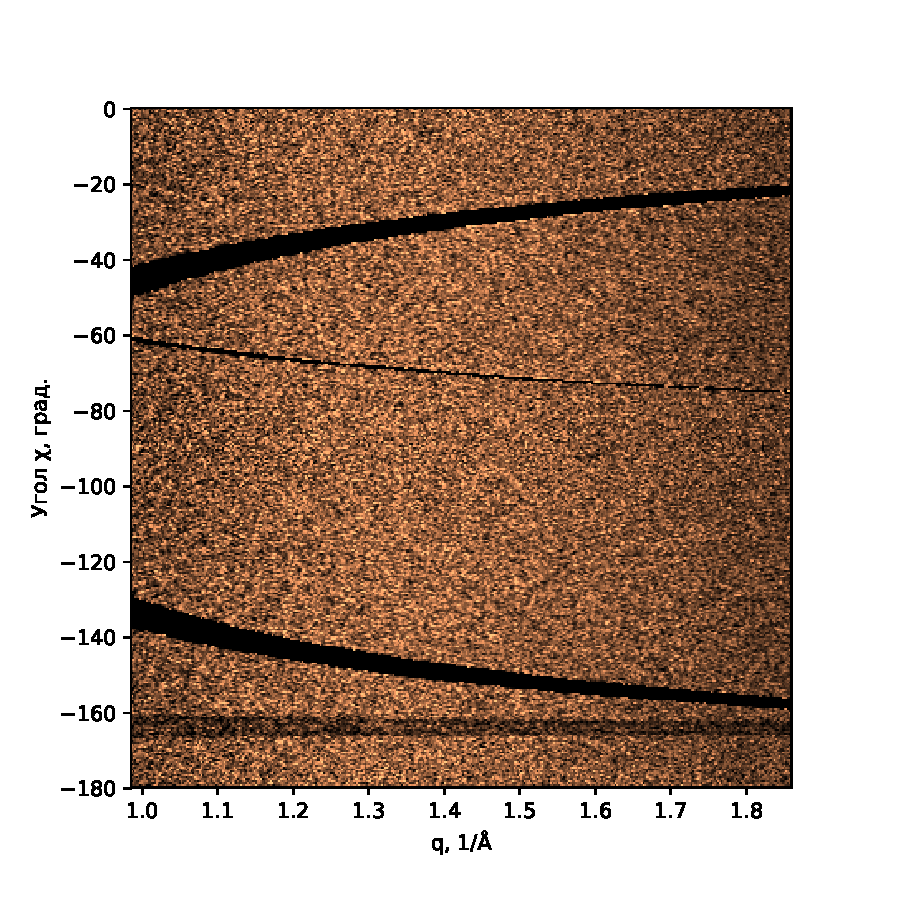
\includegraphics[width=0.5\linewidth]{fig/azim-amo.pdf}
&
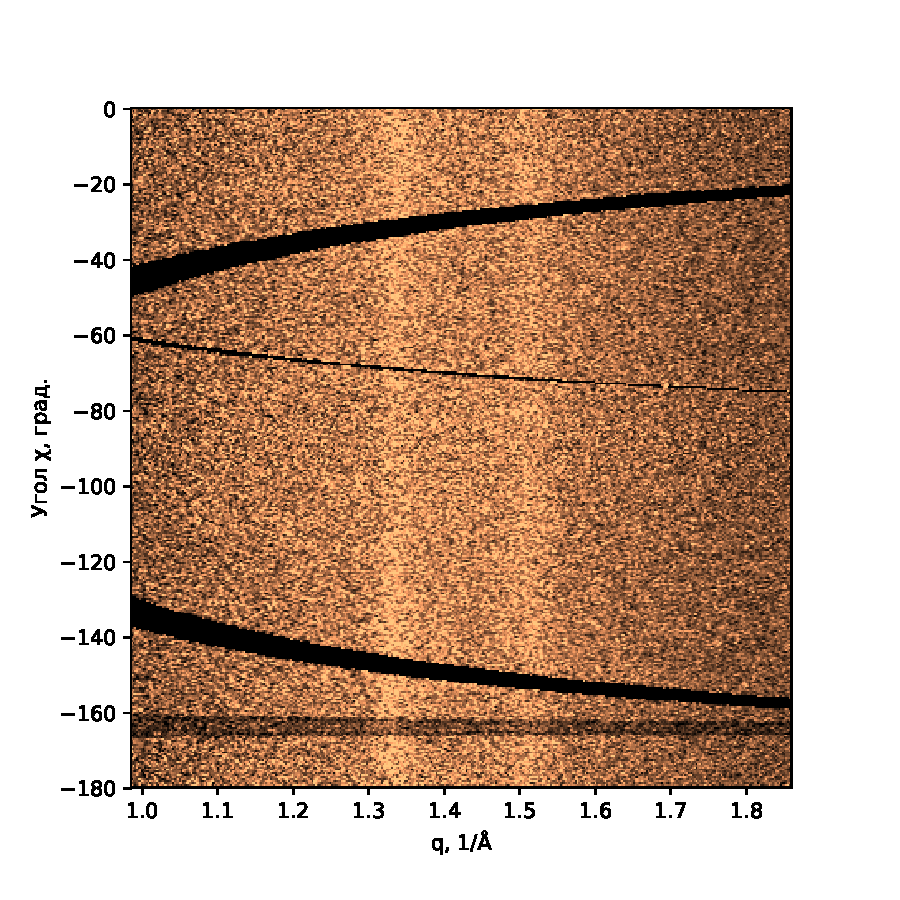
\includegraphics[width=0.5\linewidth]{fig/azim-cryst.pdf}
\end{tabular}
\caption{Фрагменты дифрактограмм (в координатах $(q,\chi)$) в аморфной (слева) и кристаллической (справа) областях.}
\label{fig:azim}
\end{figure}

	

	
	Различие в сигналах кристаллических и аморфных областей хорошо видно на фрагментах дифрактограмм, преобразованных к полярной системе координат, представленных на рис. \ref{fig:azim}. 
	Как видно из рисунка, наличие кристаллической фазы приводит к появлению  дифракционных пиков, в то время как рассеяние на чисто аморфных участках дает только так называемое аморфное гало.
	
В результате азимутального интегрирования получаются одномерные профили дифракции, как, например, профиль на рис.  \ref{fig:waxs_profile}.

		\begin{figure}[h]
    \centering
    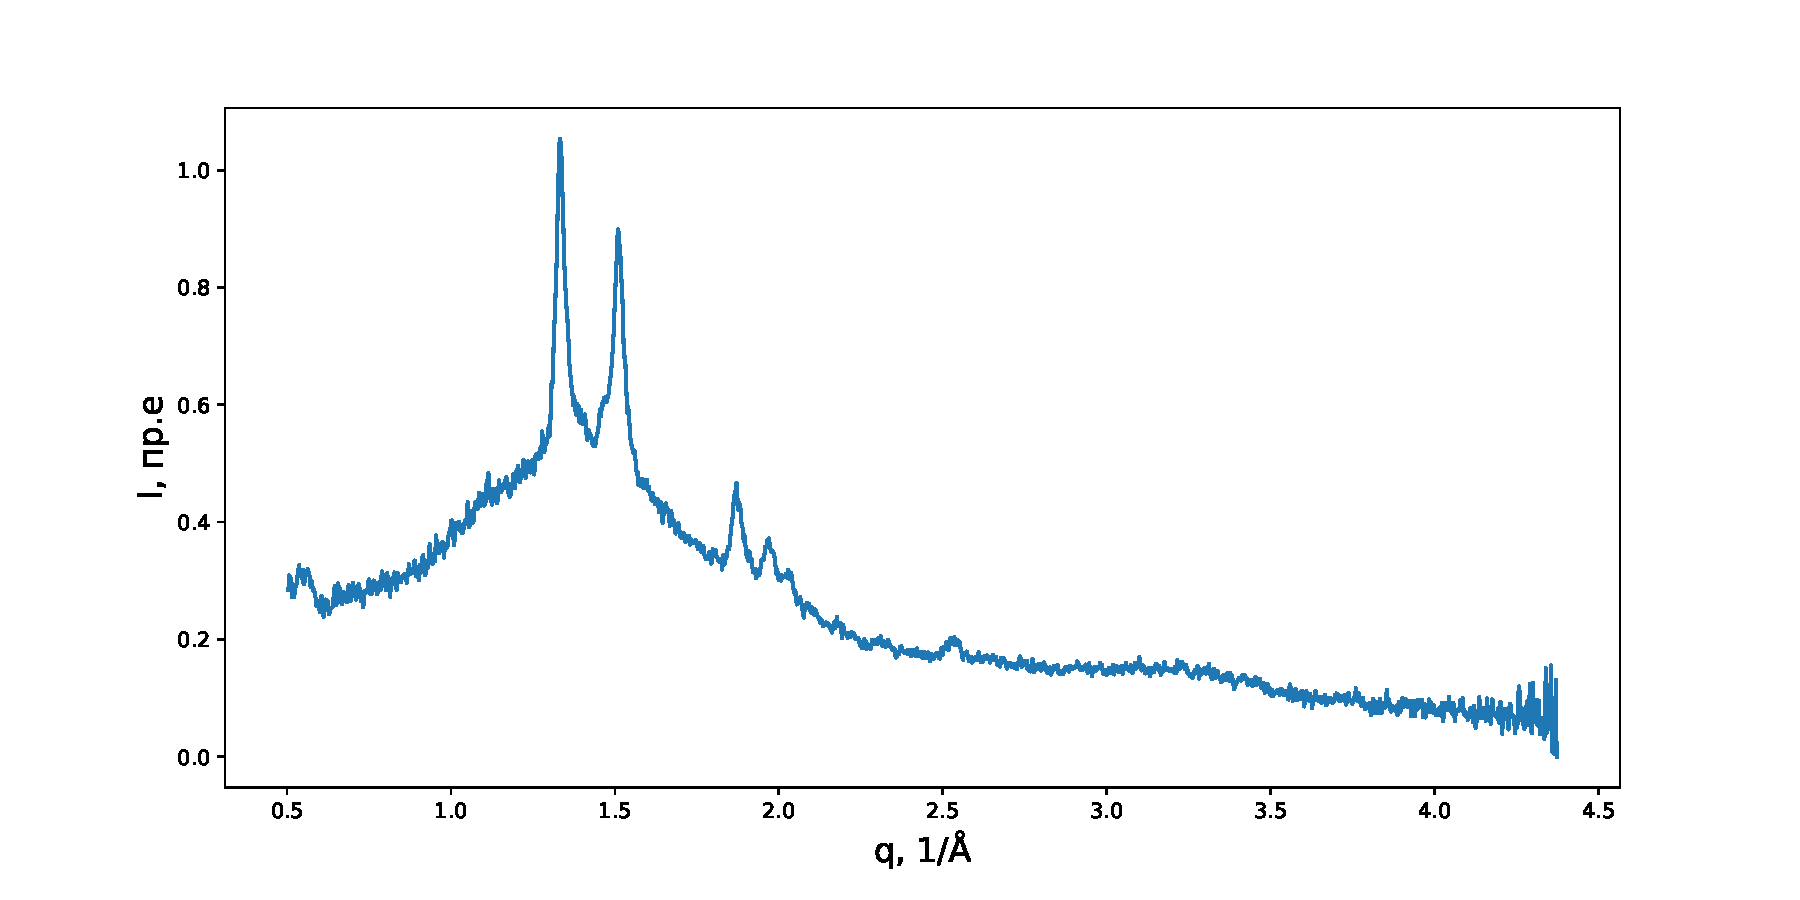
\includegraphics[width=\linewidth]{fig/profile.pdf}
    \caption{Картина дифракции в частично-кристаллической области после азимутального интегрирования}
    \label{fig:waxs_profile}
\end{figure}
	

\subsection{Вычитание фона}

	
			\begin{wrapfigure}[4]{l}{0.4\linewidth}
\singlespacing
\vspace{-35px}
%  \begin{center}
    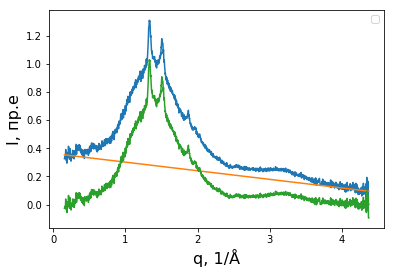
\includegraphics[width=\linewidth]{fig/base.png}
    \vspace{3px}
    \caption{Вычитание фона}
    \label{fig:base}
%  \end{center}
\end{wrapfigure}


Фоновый сигнал, не относящийся к рассеянию на изучаемом образце, приближенно аппроксимируется прямой, как показано на рис. \ref{fig:base}.



\section{Распознавание сигнала аморфной фазы}

	
	Для расчета индекса кристалличности при обработке данных дифракции необходимо распознание кристаллических пиков и сигнала от аморфной фазы.
	В отличие от обычного фона, широкие пики рассеяния от аморфной фазы нельзя определить один раз для всех измерений, так как его форма зависит от степени кристалличности. Таким образом, его оценку необходимо проводить для каждого профиля отдельно.
	Стандартные алгоритмы для автоматического распознавания фона, основанные на полиномиальной аппроксимации, показали себя неэффективными в нашем случае. Распознавание кристаллических пиков и аморфного фона производилось с помощью фильтра "rolling ball". В рентгеноструктурном анализе он как правило применяется к двумерным дифрактограммам кристаллических материалов, как например, в работе \cite{ball2018}. Однако подходящая реализация для одномерных профилей, не представлена в открытых источниках. Ниже (листинг \ref{lst:ball}) приведена реализация алгоритма для одномерных профилей на языке Python, которая применяется далее для определения кристалличности исследуемых образцов. Идеи для реализации были позаимствованы из работы \cite{ball-code}. Остальные процедуры обработки данных также производилось с помощью Python и представлены в \cite{git}.
	 
\vspace{5px}
	\begin{lstlisting}[language=Python, caption= Реализация распознавание кристаллических пиков по алгоритму "rolling ball", label={lst:ball}]
import numpy as np

def rolling_ball(profile, r):
    #r - ball radius
    #profile - 1D profile, smoothed
    t1 = np.full(profile.shape[0], np.amax(profile), dtype=np.float32)
    for i in range (t1.shape[0]):
        for j in range(-r,r):
            if ((i+j)>0 and (i+j)<t1.shape[0]):
                if(t1[i]>profile[i+j]):
                    t1[i]=profile[i+j]
                    
    t2 = np.zeros(profile.shape[0],dtype=np.float32)
    count = np.zeros(profile.shape[0],dtype=np.float32)
    back = np.zeros(profile.shape[0],dtype=np.float32) 
    
    for i in range(t2.shape[0]): 
        for j in range(-r,r):
            if ((i+j)>0 and (i+j)<t2.shape[0]):
                t2[i]+=t1[i+j]
                count[i]+=1
        back[i] = t2[i]/count[i]
    return back
 

\end{lstlisting}
\vspace{5px}

	Принцип действия алгоритма проиллюстрирован на рис. \ref{fig:ball}. 
	Его можно представить как круг заданного радиуса, который "катится"  под графиком \cite{ball2018}.Траектория его центра образует линию, которая и вычитается из начального профиля. 
		\begin{figure}[ht]
	    \centering
	    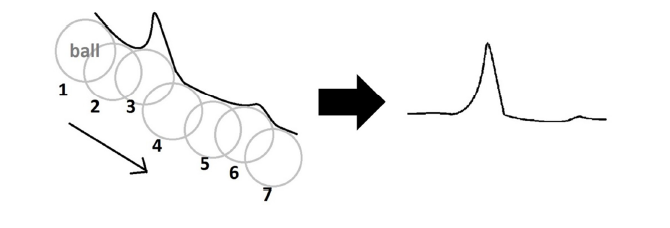
\includegraphics[width=\linewidth]{fig/ball.PNG}
	    \caption{Процедура вычитания фона.}
	    \label{fig:ball}
	\end{figure}

	
	Пики, чья ширина меньше радиуса круга, не вычитаются, и остаются в конечном профиле. Так, алгоритм позволяет убирать широкий сигнал рассеяния  на аморфной фазе, и оставлять только узкие кристаллические пики (рис. \ref{fig:ball-profile}).
	
	
	\begin{figure}[ht]
	    \centering
	    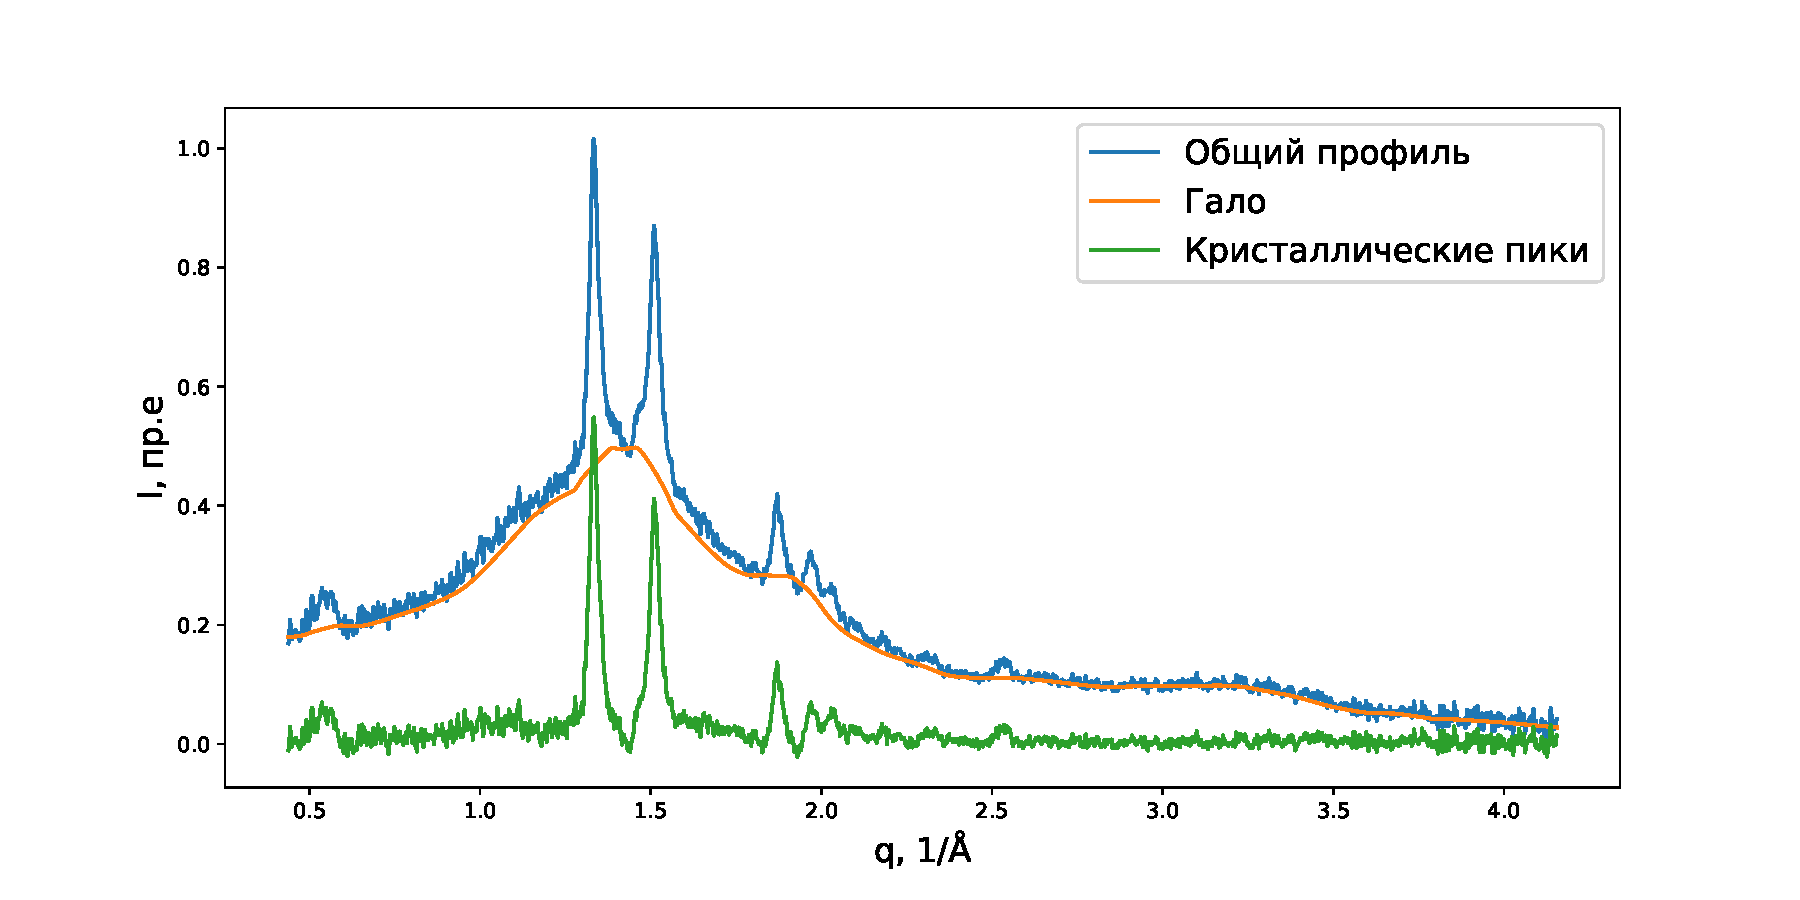
\includegraphics[width=\linewidth]{fig/ball-profile.pdf}
	    \caption{Распознавание аморфного гало}
	    \label{fig:ball-profile}
	\end{figure}



\section{Картография образцов}

\subsection{Порошки}

По данным оптической микроскопии, размеры частиц порошка составляют $5.8\pm 2.8$ мкм,и имеют мономодальное распределение. Составление карт кристалличности образцов показывает, что сами порошки состоят из частичнокристаллических частиц заявленных размеров, с индексом кристалличности около 0.1. На рис.\ref{fig:powder} показана микрограмма частиц порошка, а также карты кристалличности для исследуемых порошковых образцов.


	\begin{figure}[h]
	    \centering
	    \begin{tabular}{ccc}
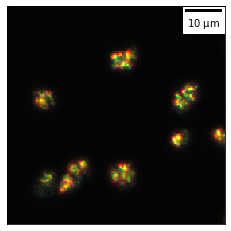
\includegraphics[width=0.26\linewidth]{fig/powder_optic.png}
&
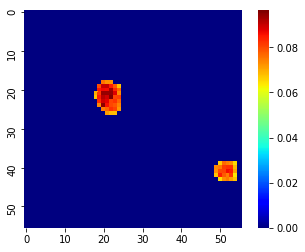
\includegraphics[width=0.33\linewidth]{fig/1416map.png}
&
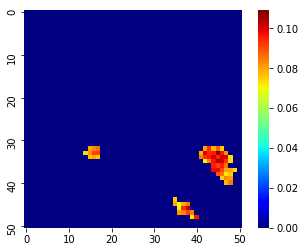
\includegraphics[width=0.33\linewidth]{fig/1434map.png}
\end{tabular}
	    \caption{Отдельные частицы}
	    \label{fig:powder}
	\end{figure}
	
Графики на рис. \ref{fig:var-profile} показывают, как изменяется интенсивность кристаллических пиков в различных областях карты: месте отсутсвия образца, не периферии и в центре частицы.

\begin{figure}[h]
    \centering
    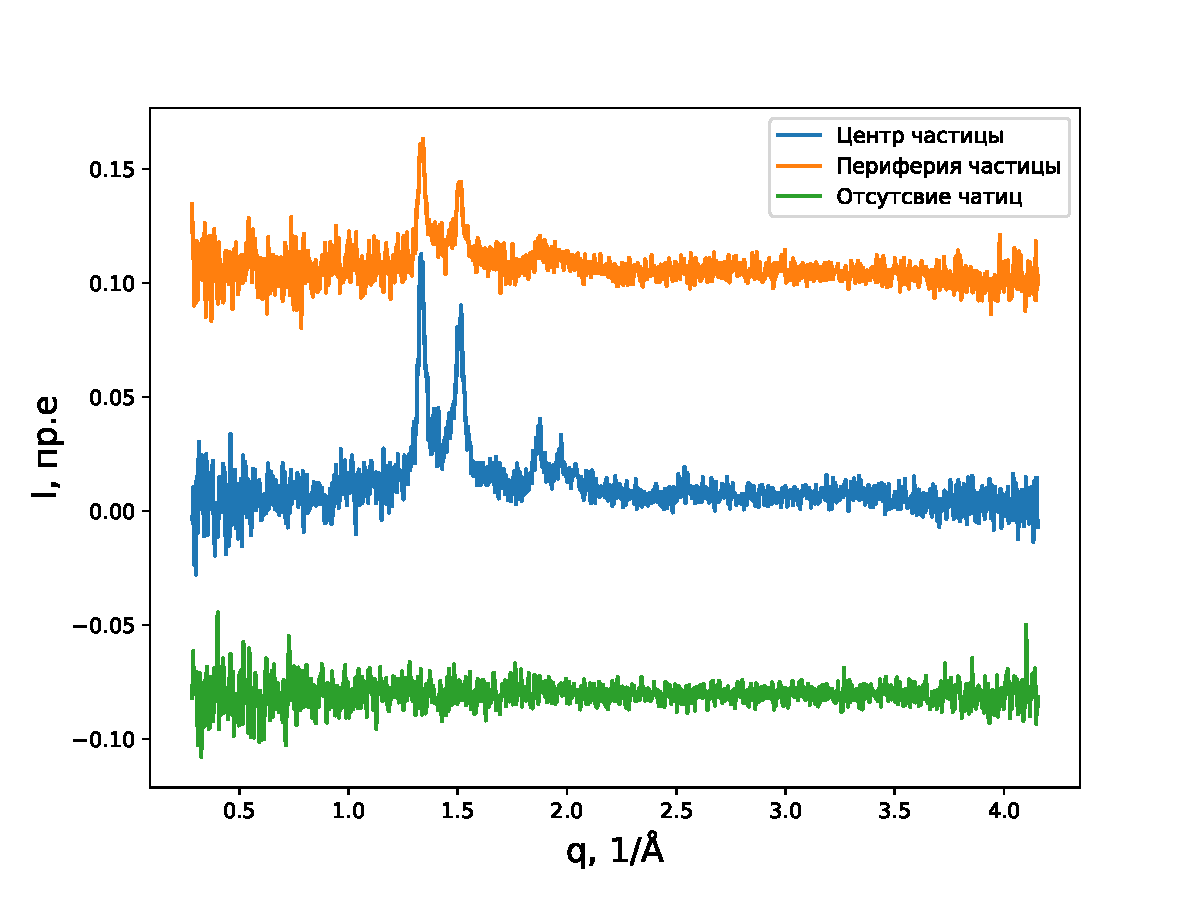
\includegraphics[width = \linewidth]{fig/var-profile.pdf}
    \caption{Сигнал кристаллической фазы в разичных областях карты кристалличности частиц порошка}
    \label{fig:var-profile}
\end{figure}

	
		\begin{figure}[h]\centering
\begin{tabular}{cc}
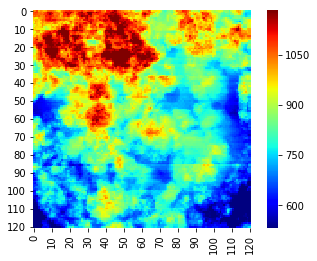
\includegraphics[width=0.5\linewidth]{fig/example72.png}
&
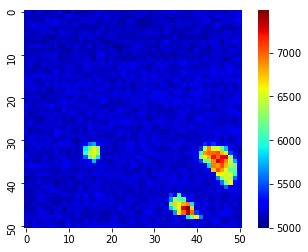
\includegraphics[width=0.5\linewidth]{fig/example1434.png} \\
\end{tabular}
\caption{Карты кристалличности}
\label{fig:maps_powder}
\end{figure}
	
	
	
%\section{Расчет характеристик}

	%Заключение
	\chapter*{Заключение}
	\addcontentsline{toc}{chapter}{Заключение}
	\section{Список результатов}
\section{Планы на будущее}

CNT was added in Polyamide 12 (PA12) in order to improve the
mechanical behaviors [60]. The laser sintered parts had 13% greater
flexural modulus, 10.9% higher flexural strength, and 54% larger
Young’s modulus. \cite{comp-review}

Furthermore, simulation results on
laser sintering of PA12-CNT suggested that inclusion of CNT helps
the laser heat to be conducted wider and deeper into the powder
bed. The result of these simulations can be observed in Fig. 19 [79].

СЛС можно делать с композитами, котрые на нейлоне показали улучшение механических свойств и уменьшение пористости
\cite{sls-composite}

Вроде как есть проблемы с тем, чтоб ыполучить композитный порошок нормальной формы \cite{sls-powder-problem}



\section{Благодарности}

	
	%Библиография
	\addcontentsline{toc}{chapter}{Литература}
	\input{6-biblio.tex}
	
	
	\chapter*{Приложение}
		
	Полную версию смотрите на гитхабе.
	
	Хотя сюда лучше вставить тех-файлы!

\end{document}